\section{Model Validation}

\begin{frame}
  \begin{center}
    {\bf Part III.b -- Model Validation}
  \end{center}
\end{frame}

\begin{frame}{Assumptions of the Null Hypothesis Statistical Testing}
  Notice that the \emph{NHST} approach adpts a number of assumptions, both statistical and technical:

  \begin{itemize}
    \item {\bf The mean is a good measure for the question of interest.}\\
    (i.e., the variance is small enough, the weigths of packages are indepentent, customers usually purchase many packages, so individual extreme values are not important, etc);\bigskip

    \item {\bf The sample is representative of our population of interest.}\\
    (i.e., the packages are from regular production (not specially produced for this test), they are not tampered with, etc)\bigskip

    \item {\bf The contents of the packages are actually chocolate}\\
    (the weight of the package is not a significant part of the measured weight, etc);\bigskip

    \item ... and others ...
  \end{itemize}
\end{frame}

\begin{frame}{Assumptions of the Null Hypothesis Statistical Testing}{Statistical Assumptions}

  More specifically, the testing and analysis procedure that we studied (calculation of test statistic, etc), assumes that our experiment can be described by a specific model:\bigskip

  \begin{itemize}
    \item The sample distribution follows a normal curve (Assumption of Normality);
    \item The observations in the sample are independent (Assumption of Independence);
    \item The variance is constant (Assumption of variance);
    \item etc..
  \end{itemize}\bigskip

  It is important to validate these assumptions, to make sure that our test, analysis and conclusions are valid!
\end{frame}

\subsection{Assumptions}
\begin{frame}{Assumption of Normality}
  The assumption of Normality is required by the {\bf z} and {\bf t} tests described in this lecture:\medskip

  \begin{block}{}
    "\emph{The Assumption of Normality (note the upper case) that underlies parametric stats does not assert that the observations within a given sample are normally distributed, nor does it assert that the values within the population (from which the sample was taken) are normal. This core element of the Assumption of Normality asserts that {\bf the distribution of sample means (across independent samples) is normal}.}"\bigskip

    \hfill J. Toby Mordkoff, 2011\footnote{J.T. Mordkoff, The assumption(s) of normality: \url{http://goo.gl/Z3w8ku}}
  \end{block}
\end{frame}

\begin{frame}{The normality assumption}{Visual Inspection}
  If we cannot assume the conditions for the CLT \emph{a priori},
  then we can perform normality tests on the data.

  \begin{columns}
    \column{0.6\textwidth}
      The {\bf QQ plot} (quantile-quantile plot) plots the quantiles of two data sets against each other. If one of the data-sets is the theoretical normal quantiles, this plot can help visualize deviations from normality.\bigskip
    \column{0.4\textwidth}
      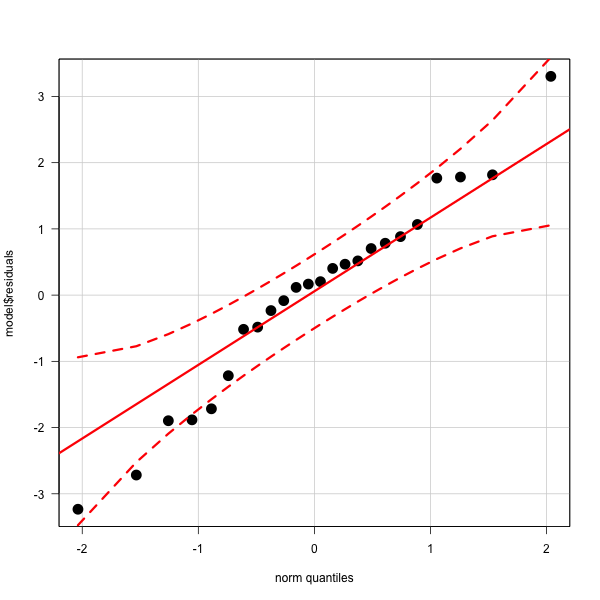
\includegraphics[width=\textwidth]{../img/qq_plot}
  \end{columns}
\end{frame}

\begin{frame}{The normality assumption}{Normality Tests}
  You can also perform statistical tests on the assumption of normality:
  \begin{itemize}
    \item {\bf Shapiro-Wilk;\hfill <- recommended for this course;}
    \item Anderson-Darling;
    \item Lilliefors / Kolmogorov-Smirnov;
  \end{itemize}\bigskip

  These procedures use different aspects of the sample distribution to test the following hypotheses:
  \begin{itemize}
    \item $H_0$: The population is normal;
    \item $H_1$: The population is not normal;
  \end{itemize}\bigskip

  In this case, rejection of the null hypothesis suggests evidence that the {\bf sample} came from a non-normal distribution. Although, for a large enough sample, the CLT might still guarantee a normally distributed {\bf sample mean estimate}, a visual investigation of the distribution of sample's observations is very important in this case.
\end{frame}

\begin{frame}{The independence assumption}
  The strongest assumption used for the t-test is the {\bf independence assumption}. This assumption means that the value of observations are not dependent (biased) on the values of other observations.\bigskip

  Example of independence violation:
  \begin{itemize}
    \item You measure the speed of a robot in 10 trials. However, because the battery is low, the speed will progressively decay;
    \item You measure the accuracy of an algorithm in predicting 20 time series curves. However, 5 of those curves represent different instances of the same model, and are closely related to each other.
  \end{itemize}\bigskip

  In general, we want to guarantee the independence assumption through careful experiment design. The {\bf Durbin-Watson} test can be used to detect auto-correlation, but it is sensitive to the order of observations.
\end{frame}
